\documentclass{beamer}%[handout]

\mode<presentation>
{
       \usetheme{metropolis}
}
\usepackage{latexsym}
\usepackage{verbatim}
\usepackage{amssymb, amsmath}
\usepackage{graphicx, graphics,txfonts}
\usepackage{tikz-qtree}
%\usepackage{qtree}
%\usepackage{etex}
%usepackage[all]{xy}
\usepackage{color}
%\usepackage[final]{pdfpages}
\usepackage[round]{natbib}

\newcommand{\tuple}[1]{\langle #1 \rangle}
\newcommand{\norm}[1]{\left\| #1 \right\|}
\newcommand{\bin}[2]{\left(#1\atop{#2}\right)}

\graphicspath{{../figures/}}

\title{Lecture 7: Reinforcement Learning}
\author{Satchit Chatterji\\ SIAS Group, IvI, Universiteit van Amsterdam \\ \textit{\tiny{(based on a slideset by Jelle Zuidema \& Iris Proff)}}}
\institute{}
\date{Machine Learning and Language Models, 2026}

\begin{document}

\begin{frame}
\titlepage
\end{frame}

%\section{Introduction}
%\begin{frame}{Plan}
%%\tableofcontents[currentsection]
%\end{frame}

%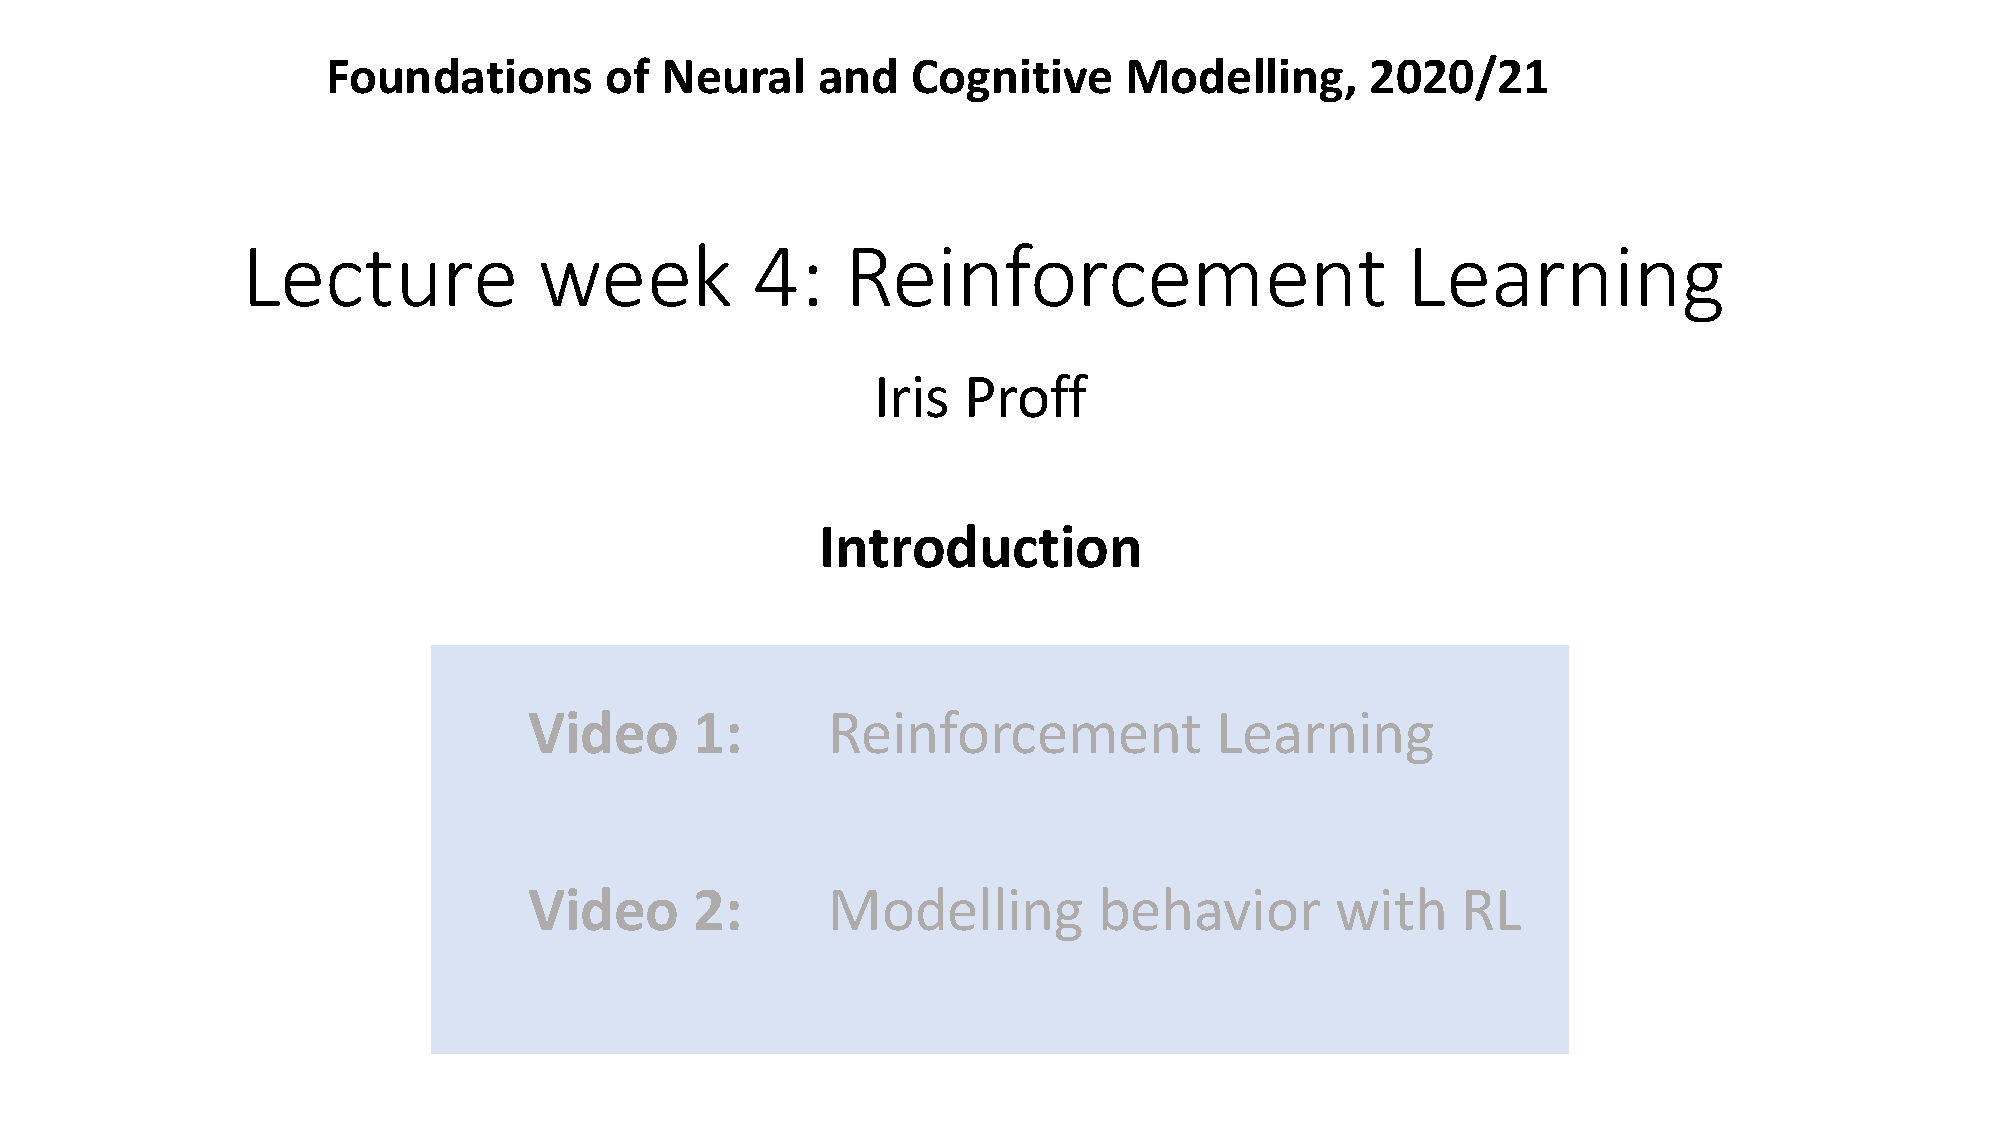
\includegraphics[page=1,width=\linewidth]{../figures/Week5_RL_slides}\\
%\includegraphics[page=2,width=\linewidth]{../figures/Week5_RL_slides}\\
%\includegraphics[page=3,width=\linewidth]{../figures/Week5_RL_slides}\\
%\includegraphics[page=4,width=\linewidth]{../figures/Week5_RL_slides}\\
%\includegraphics[page=5,width=\linewidth]{../figures/Week5_RL_slides}\\

\section{What is Reinforcement Learning?}
\begin{frame}{Plan}
\tableofcontents[currentsection]
\end{frame}

\includegraphics[page=6,width=\linewidth]{../figures/Week5_RL_slides}\\
\includegraphics[page=7,width=\linewidth]{../figures/Week5_RL_slides}\\
\includegraphics[page=8,width=\linewidth]{../figures/Week5_RL_slides}\\
\includegraphics[page=9,width=\linewidth]{../figures/Week5_RL_slides}\\
\includegraphics[page=10,width=\linewidth]{../figures/Week5_RL_slides}\\

\begin{frame}{}
\includegraphics[page=11,width=.5\linewidth,trim=0cm 0cm 17cm 3.8cm, clip]{../figures/Week5_RL_slides}\\
\pause
\begin{block}{Question 1}
Consider states $S_2$ and $S_3$ (which can you reach with action $A_1$ and $A_2$) and state $S_4$ (which you can reach from state $S_3$ by action $A_1$). How valuable are each of these states relative to eachother? Is $U(S_1)=U(S_3)$? \end{block}
\end{frame}

\begin{frame}{}
\includegraphics[page=11,width=\linewidth]{../figures/Week5_RL_slides}\\
\pause
\begin{block}{Question 2}
How do you avoid having to first learn everything about the environment/problem before you can start acting in the world?
\end{block}
\end{frame}

\section{Q-learning}
\begin{frame}{Plan}
\tableofcontents[currentsection]
\end{frame}

\includegraphics[page=12,width=\linewidth]{../figures/Week5_RL_slides}\\
\includegraphics[page=13,width=\linewidth]{../figures/Week5_RL_slides}\\

\begin{frame}{}
\includegraphics[page=14,width=\linewidth,trim=0cm 5cm 5cm 0cm, clip]{../figures/Week5_RL_slides}\\
\pause
\begin{block}{Question 3}
How do you make sure you maximize reward, both in the short term (taking advantage of your knowledge) and in the long term (extending your knowledge)?
\end{block}
\end{frame}


\begin{frame}
\includegraphics[page=15,width=\linewidth]{../figures/Week5_RL_slides}\\
\pause
Classic example: \textcolor{blue}{multi-armed bandit}
\end{frame}

\begin{frame}{Multi-armed bandit}
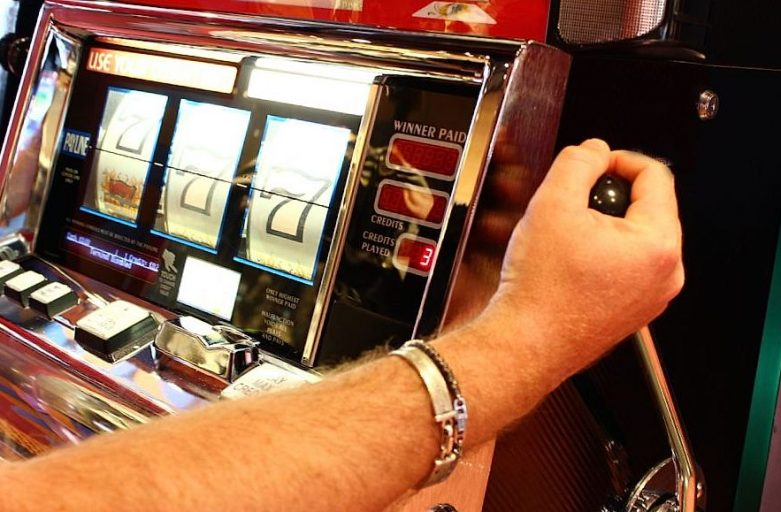
\includegraphics[width=.32\linewidth]{../figures/one-armed-bandit-slot-781x512}
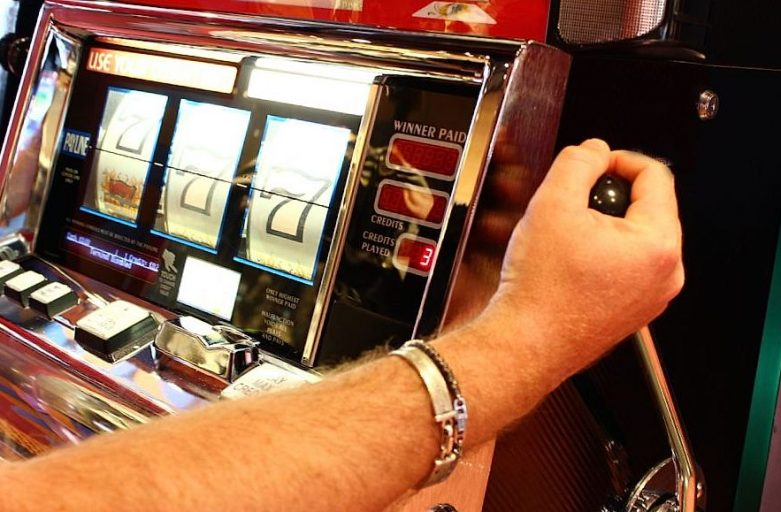
\includegraphics[width=.32\linewidth]{../figures/one-armed-bandit-slot-781x512}
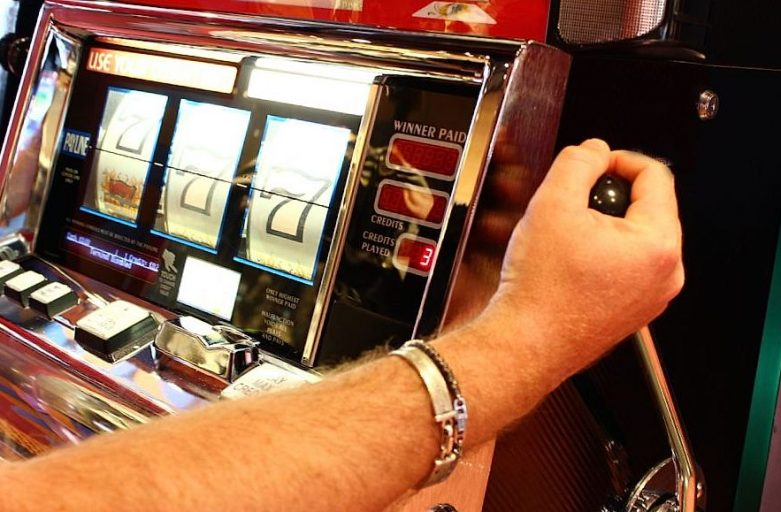
\includegraphics[width=.32\linewidth]{../figures/one-armed-bandit-slot-781x512}\\

{\small \it The name comes from imagining a gambler at a row of slot machines ("one-armed bandits"), who has to decide which machines to play, how many times to play each machine and in which order to play them, and whether to continue with the current machine or try a different machine.}
\end{frame}


\includegraphics[page=16,width=\linewidth]{../figures/Week5_RL_slides}\\
\includegraphics[page=17,width=\linewidth]{../figures/Week5_RL_slides}\\

\section{RL in the brain}
\begin{frame}{Plan}
\tableofcontents[currentsection]
\end{frame}
\includegraphics[page=18,width=\linewidth]{../figures/Week5_RL_slides}\\

\section{Model-based RL}
\begin{frame}{Plan}
\tableofcontents[currentsection]
\end{frame}

\includegraphics[page=19,width=\linewidth]{../figures/Week5_RL_slides}\\
\includegraphics[page=20,width=\linewidth]{../figures/Week5_RL_slides}\\

\includegraphics[page=21,width=\linewidth]{../figures/Week5_RL_slides}\\
\includegraphics[page=22,width=\linewidth]{../figures/Week5_RL_slides}\\
%\includegraphics[page=23,width=\linewidth]{../figures/Week5_RL_slides}\\


\section{Extensions of Q-learning}
\begin{frame}{Plan}
\tableofcontents[currentsection]
\end{frame}

\includegraphics[page=38,width=\linewidth]{../figures/Week5_RL_slides}\\

\section{Deep RL}

\begin{frame}{Plan}
\tableofcontents[currentsection]
\end{frame}


\begin{frame}{Deep Reinforcement Learning}
\centerline{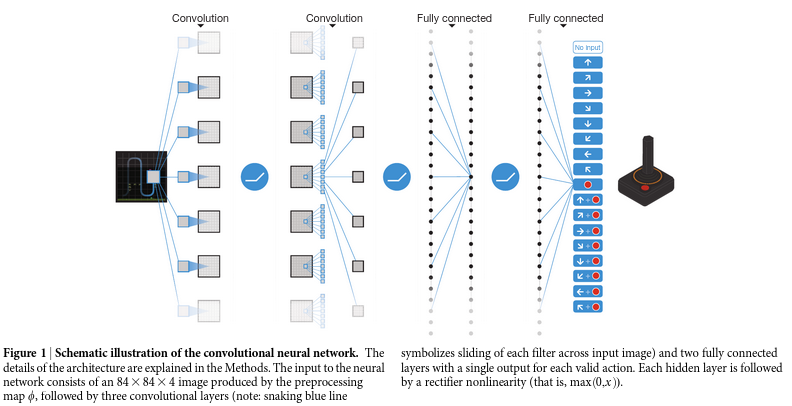
\includegraphics[width=\linewidth,trim=3cm 2.5cm 3cm 0cm,clip]{../figures/deepRLscheme_mnih_etal15nature}}
\end{frame}

\begin{frame}{Deep Q-Learning (Mnih et al. 2015)}
\begin{itemize}
    \item Replace Q-table with a  neural network $Q$, with weights $\theta$; use it to compute Q-value of current state
    \item Make a copy of the Q-network (the \emph{target-network} $\hat{Q}$); use it to compute Q-value of target states
    \item Learn in batches: act in the world (choose actions using $\epsilon$-greedy) and gather data 
    \item Optimize Q-network (mimize prediction error) via gradient descent on a batch of observations
    \item Occasionally copy $Q$ into $\hat{Q}$
\end{itemize}
\end{frame}

\begin{frame}{Deep Q-Learning (Mnih et al. 2015)}
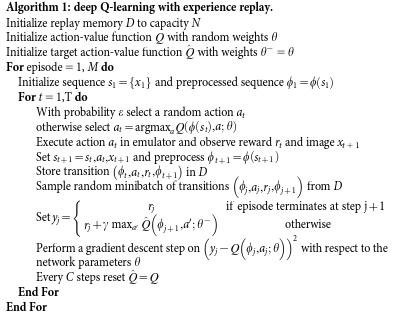
\includegraphics[height=.8\textheight,trim=0cm 0cm 0cm 0cm,clip]{../figures/deepRL_mnih_etal15nature}\\
\end{frame}

\begin{frame}{Deep Q-Learning (Mnih et al. 2015)}
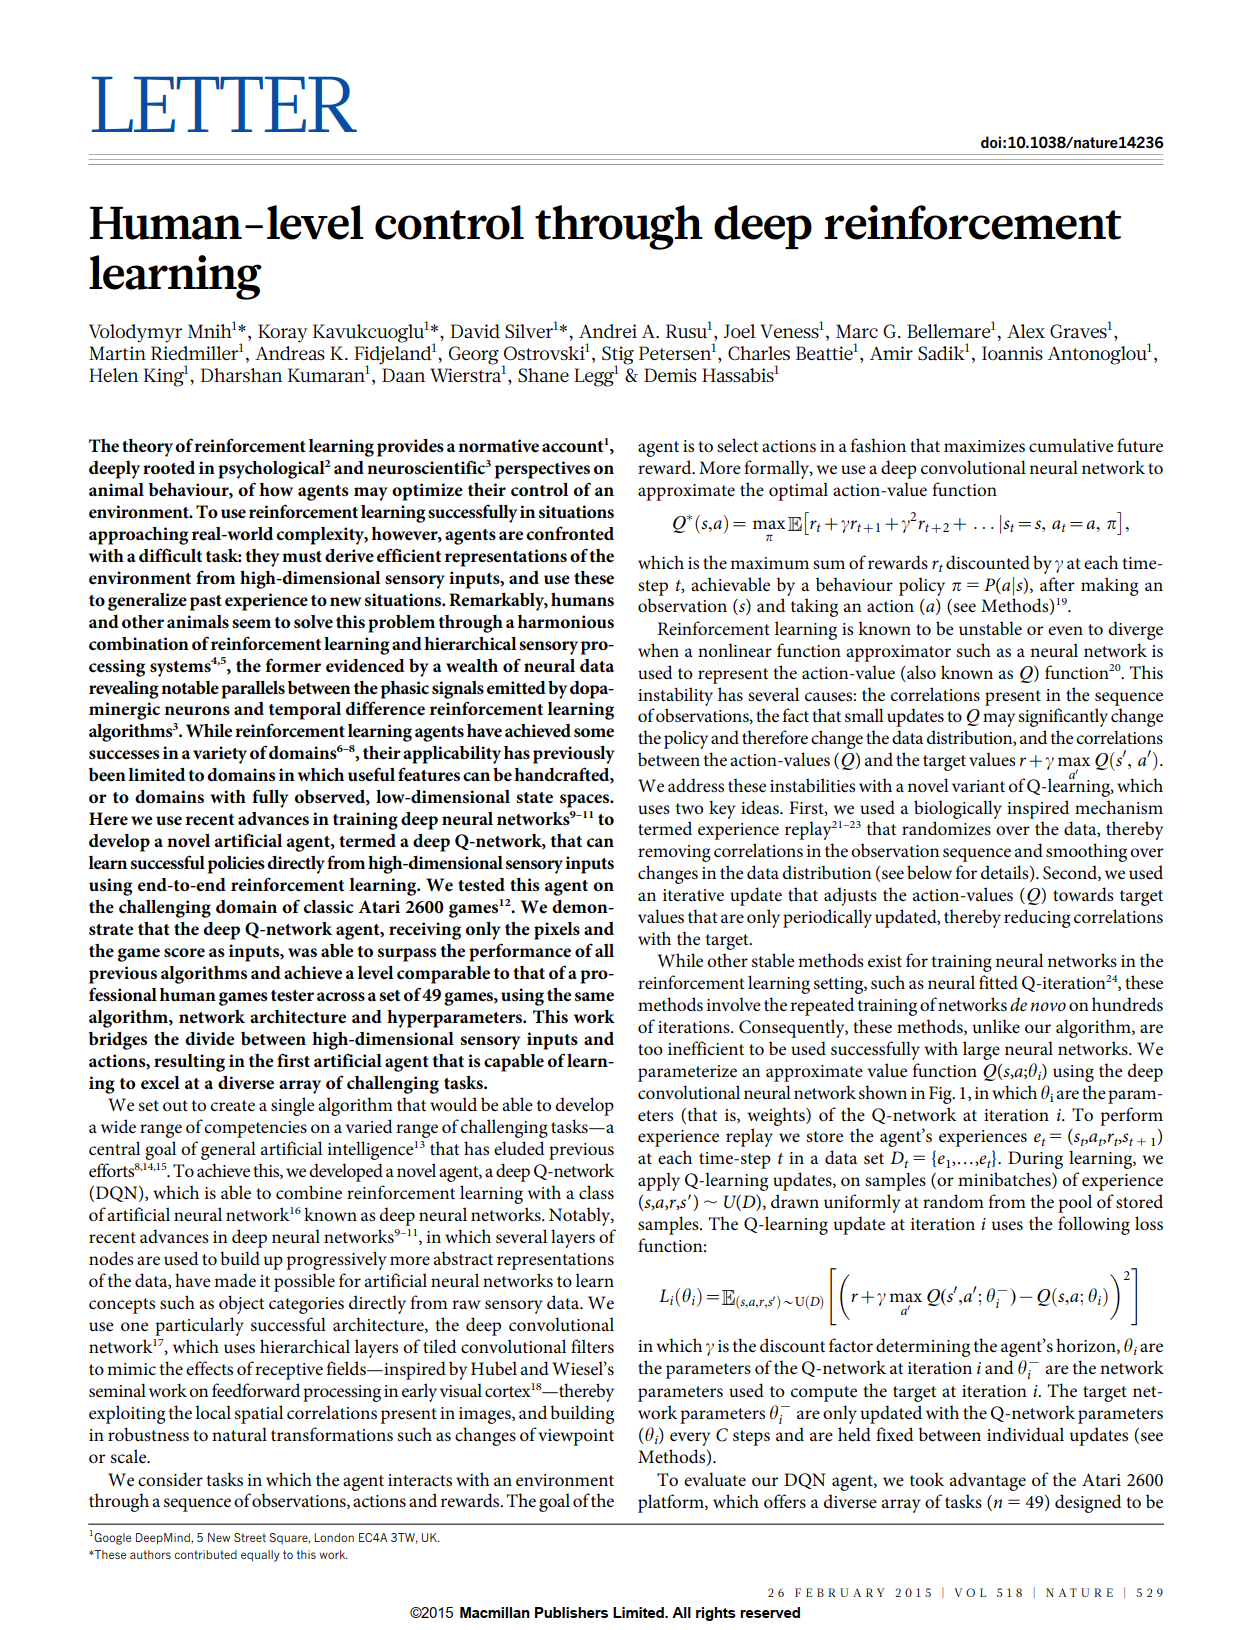
\includegraphics[height=.75\textheight,trim=0cm 0cm 0cm 0cm,clip]{../figures/deepRL_minh15-firstpage}
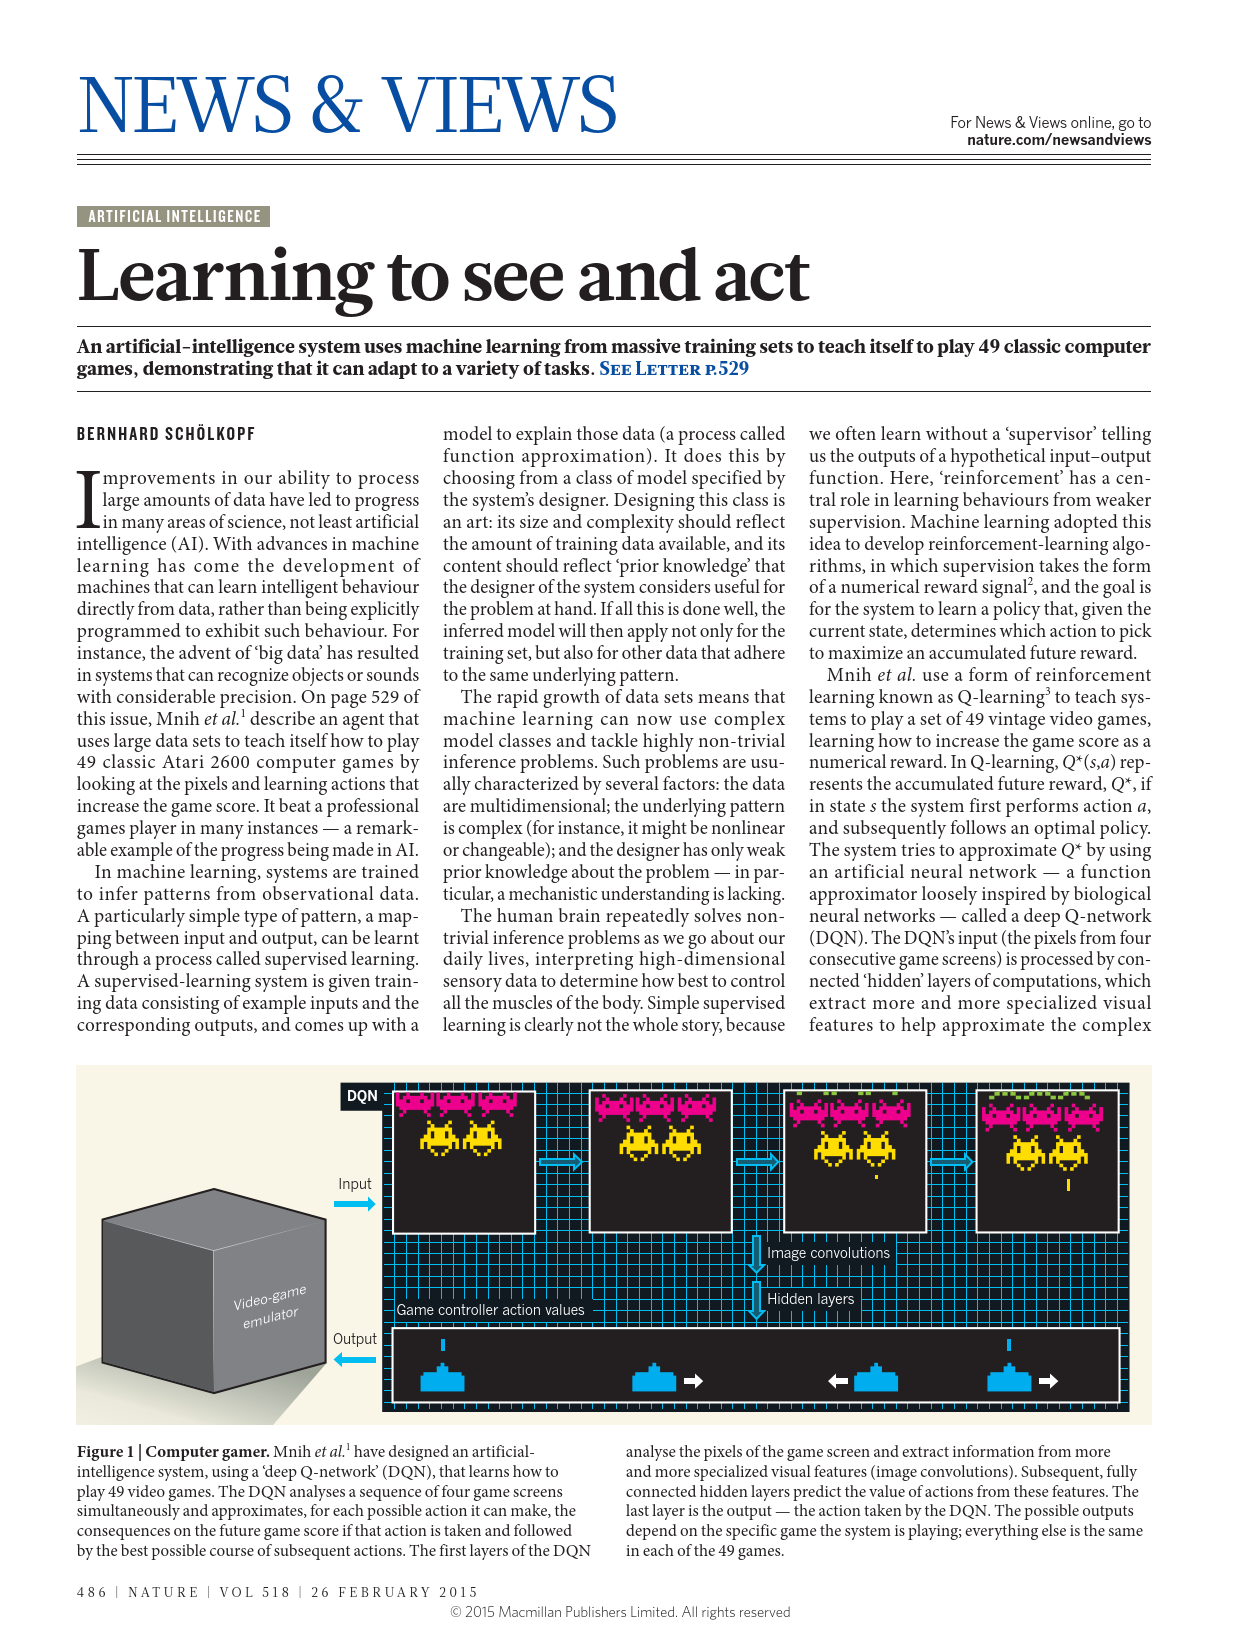
\includegraphics[height=.75\textheight,trim=0cm 0cm 0cm 0cm,clip]{../figures/learningtoseeandact}\\
\end{frame}

\begin{frame}{Deep Reinforcement Learning}
\includegraphics[page=39,width=.9\linewidth,trim=0cm 0cm 9cm 6.5cm,clip]{../figures/Week5_RL_slides}\\
\url{https://wiki.pathmind.com/deep-reinforcement-learning}
\end{frame}




\end{document}
